\documentclass{beamer}
\setbeamertemplate{navigation symbols}{}
\setbeamertemplate{bibliography item}[text]

\usepackage{beamerthemeshadow}
\usepackage{amsmath}
\usepackage{amssymb}
\usepackage{graphicx}
\graphicspath{ {./images/} }
\begin{document}
\title{Total unimodular matrices (TU): examples, properties}  
\author{Coman Florin-Alexandru}

\begin{frame}
\titlepage
\end{frame}

\begin{frame}\frametitle{Table of contents}\tableofcontents
\end{frame}

\section{Total unimodular matrices (TU)}
\subsection{Definition}
\begin{frame}\frametitle{Total unimodular matrices}
\begin{block}{Definition}
A Matrix A is \textbf{totally unimodular} (TU) if the determinant of every square submatrix of $A$ (also called minor of $A$) has value −1, 0 or 1. Or mathematically \\
\centerline{$A TU \Longleftrightarrow \forall$ square submatrix $K$, $det(K) \in \lbrace -1, 0, 1 \rbrace$}
\end{block}
\begin{block}{Example}
$\begin{pmatrix}
1& 1& 0 \\
0& 1& 1 \\
0& 0& 1
\end{pmatrix}$ is a TUM, as its determinant is equal to 1.
\end{block}
\end{frame}

\section{Properties}
\subsection{Properties}
\begin{frame}\frametitle{Properties}
\begin{block}{Proposition 1}
If $A \in TU, A_j$ be the $j$-th row of $A$, then \\
\centerline{$A^T \in TU$}
\end{block}
\begin{block}{Proof}
$det(M) = det(M^T)$
\end{block}
\end{frame}

\begin{frame}\frametitle{Properties}
\begin{block}{Proposition 2}
If $A \in TU, A_j$ be the $j$-th row of $A$, then \\
\centerline{$A'$ is a submatrix of $A$, then $A' \in TU$}
\end{block}
\begin{block}{Proof}
square submatrix of $A'$ is also square submatrix of $A$
\end{block}
\end{frame}

\begin{frame}\frametitle{Properties}
\begin{block}{Proposition 3}
If $A \in TU, A_j$ be the $j$-th row of $A$, then \\
\centerline{$\begin{bmatrix}
0 \\
A_1 \\
A_2 \\
. \\
. \\
. \\
A_m
\end{bmatrix}$}
\end{block}
\begin{block}{Proof}
The submatrices that doesn't contain the first row has corresponding submatrix in $A$, ones that does contain the first row has determinant 0.
\end{block}
\end{frame}

\begin{frame}\frametitle{Properties}
\begin{block}{Proposition 4}
If $A \in TU, A_j$ be the $j$-th row of $A$, then \\
\centerline{If $A$ is a square matrix, then $A^{-1} \in TU$}
\end{block}
\begin{block}{Proof}
If $B = A^{-1}$, then we have an equality between minors: \\
\centerline{$B(I, J) = \pm \frac{A(J^c, I^c)}{det(A)},$}
for every subsets $i, J \subset [[1, n]]$ of same cardinals. This formula generalizes that giving the entries of $A^−1$ in terms of minors of $A$.
\end{block}
\end{frame}

\begin{frame}\frametitle{Properties}
\begin{block}{Proposition 5}
If $A \in TU, A_j$ be the $j$-th row of $A$, then \\
\centerline{If $A'$ is formed by row swapping of $A$, then $A' \in TU.$}
\end{block}
\begin{block}{Proof}
Consider we switched row $i$ and $j$. Consider any submatrix, if it doesn't contain row $i$ or $j$, then it still has determinant −1,0,1. If it contain both row $i$ and $j$, then the determinant is just the negation when the rows are switched back. If it only contain one of row $i$ and $j$, wlog let it be $i$, then it has the rows in order $a_1, ..., a_k, i, a_{k+1}, ..., a_l$, then there is a submatrix in $A$ using the rows in sequence $a_1, ..., a_j, i, a_{j+1}, ..., a_l$, and the absolute value of their determinants are equal.
\end{block}
\end{frame}

\begin{frame}\frametitle{Properties}
\begin{block}{Proposition 6}
If $A \in TU, A_j$ be the $j$-th row of $A$, then \\
\centerline{If $A'$ id formed by multiplying by -1, 0 or 1 to a row, then $A' \in TU$}
\end{block}
\begin{block}{Proof}
multiply by a constant to preserve the −1,0,1 properties, then use the argument similar as above, note the determinant of the submatrix can change only by sign.
\end{block}
\end{frame}

\section{Examples}
\subsection{Bipartite Graphs}
\begin{frame}\frametitle{Bipartite Graphs}
\begin{block}{}
Let $A$ be the incidence matrix of a bipartite graph. Each row $i$ represents a vertex $v(i)$, and each column $j$ represents an edge $e(j)$. $A(ij) = 1$ if and only if edge $e(j)$ is incident to $v(i)$.
\begin{figure}[h]
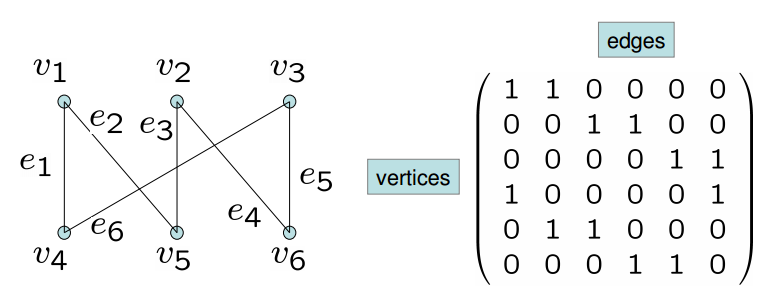
\includegraphics[width=8cm]{picture1}
\end{figure}
\end{block}
\end{frame}

\begin{frame}\frametitle{Bipartite Graphs}
\begin{block}{}
The incidence matrix $A$ of a bipartite graph is totally unimodular.
\end{block}
\begin{block}{Proof I} 
Consider an arbitrary square submatrix $A'$ of $A$. Our goal is to show that $A'$ has determinant ­1,0, or +1. \\
\textbf{Case 1.} $A'$ has a column with only 0. \\
\centerline{Then $det(A') = 0$.}
\textbf{Case 2.} $A'$ has a column with only one 1. \\
\centerline{$A' = \begin{pmatrix}
1& a^T \\
0& A''
\end{pmatrix}$}
By induction, $A''$ has determinant -1, 0, or +1. And so does $A'$
\end{block}
\end{frame}

\begin{frame}\frametitle{Bipartite Graphs}
\begin{block}{Proof II}
\textbf{Case 3.} Each column of $A'$ has exactly two 1. \\
\centerline{We can write $A' = \begin{pmatrix}
A^{up} \\
A^{down}
\end{pmatrix}$}
Since the graph is bipartite, each column has one 1 in $A^{up}$ and one 1 in $A^{down}$. \\
So, by multiplying +1 on the rows in $A^{up}$ and ­1 on the columns in $A^{down}$, we get that the rows are linearly dependent, and thus $det(A') = 0$, and we’re done.
\begin{figure}[h]
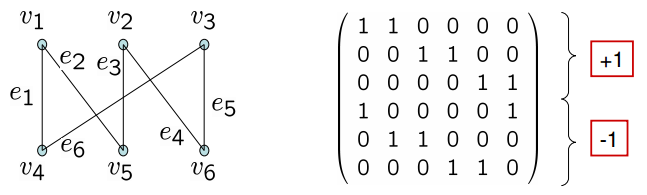
\includegraphics[width=7cm]{picture2}
\end{figure}
\end{block}
\end{frame}

\subsection{Directed Graphs}
\begin{frame}\frametitle{Directed Graphs}
\begin{block}{}
Let $A$ be the incidence matrix of a directed graph. Each row $i$ represents a vertex $v(i)$, and each column $j$ represents an edge $e(j)$. \\
$\bullet$ $A(ij) = +1$ if vertex $v(i)$ is the tail of edge $e(j)$. \\
$\bullet$ $A(ij) = ­-1$ if vertex $v(i)$ is the head of edge $e(j)$. \\
$\bullet$ $A(ij) = 0$ otherwise.
\end{block}
\begin{block}{}
The incidence matrix $A$ of a directed graph is totally unimodular.
\end{block}
\end{frame}

\subsection{Other examples}
\begin{frame}\frametitle{Other examples}
\begin{block}{}
Unimodular matrices form a subgroup of the general linear group under matrix multiplication, i.e. the following matrices are unimodular: \\
$\bullet$ \textbf{Identity matrix} \\
$\bullet$ \textbf{The inverse of a unimodular matrix} \\
$\bullet$ \textbf{The product of two unimodular matrices} \\
\end{block}
\end{frame}

\section{Bibliography}
\begin{frame}[allowframebreaks]
\frametitle{Bibliography}
    \tiny{\bibliographystyle{abbrv} }
    \bibliography{main}
\end{frame}
\end{document}